\documentclass[10pt]{article}

\usepackage[left=1.5cm,
            right=1.5cm,
            top=2.5cm,
            bottom=2.5cm]{geometry}
\usepackage{hyperref}
\usepackage{fancyhdr}
\usepackage{titling}
\usepackage{amsmath}
\usepackage{graphicx}
\graphicspath{ {./Output/} }
\usepackage{caption}
\usepackage{subcaption}
\usepackage{array}
\usepackage{mdframed}

\title{DMML - Assignment 3}
\author{Ishita Pethkar (BMC202128), Siddhant Shah (BMC202171)}
\date{$21^{st}$ April, 2024}

\pagestyle{fancy}
\fancyhead{}
\lhead{\href{https://github.com/SidShah2953/dmml-2024}{GitHub URL}}
\chead{\thetitle}
\rhead{Ishita Pethkar, Siddhant Shah}

\begin{document}
% \thispagestyle{empty}
\maketitle
\tableofcontents

\section{General Strategy}

\subsection{The Data}
   We carry out semi-supervised learning on two datasets: Fashion MNIST and Overhead MNIST. In these datasets, images are of $28 \times 28$ pixels giving us $784$ attributes. The Fashion MNIST dataset has $60000$ training images and $10000$ test images and the Overhead MNIST data has $68152$ training images and $8520$ test images.

\subsection{Pre-processing the data}
    As the data has $784$ attributes, processing this data is difficult and increases time complexity. So we reduce the dimensions of the data by carrying out Principal Component Analysis(PCA), from $784$ to $28$.

\subsection{Semi-supervised Learning}
    We now use $k$-means clustering on our reduced-dimension data. We carry out clustering for $k = 50$ to  $k = 1000$. We then find the optimal $k$ by the Elbow Method. We then carry out semi-supervised learning as has been mentioned in Lecture 15. 
    
    We carry out three processes on each data set and compare the performances of the MLP after each:
    \begin{itemize}
        \item \emph{$K$ Representative Images}: We find the representative images for each cluster and fit our MLP model\footnote{We use the MLP model in Lecture 18.} on just these representative images.
        \item \emph{Full Propagation}: We propagate the labels of the representative images on the entire cluster and fit our MLP model on this new dataset.
        \item \emph{Partial Propagation}: We propagate the labels of the representative images on only nearest $20$ percentile points in each cluster and then fit our MLP model on this dataset.
    \end{itemize}

\newpage
\section{Results}
\subsection{Fashion MNIST}
  After clustering, optimal $k = 450$.
    \begin{table}[h]
        \begin{center}
            \begin{tabular}{|l|l|l|l|l|}
                \hline
                Model &Accuracy &Loss &Val-Accuracy &Val-Loss \\
                \hline
                Original &0.896 &0.293 &0.873 &0.352 \\
                $K$ Representative Images &0.776 &0.752 & 0.706 &0.874 \\
                Full Propagation &0.875 &0.308 &0.785 &0.662 \\
                Partial Propagation  &0.889 &0.289 &0.798 &0.624 \\
                \hline
            \end{tabular}
        \end{center}
    \end{table}
    \begin{figure}[!h]
        \centering
        \begin{subfigure}[b]{0.48\textwidth}
            \centering
            \caption{Original}
            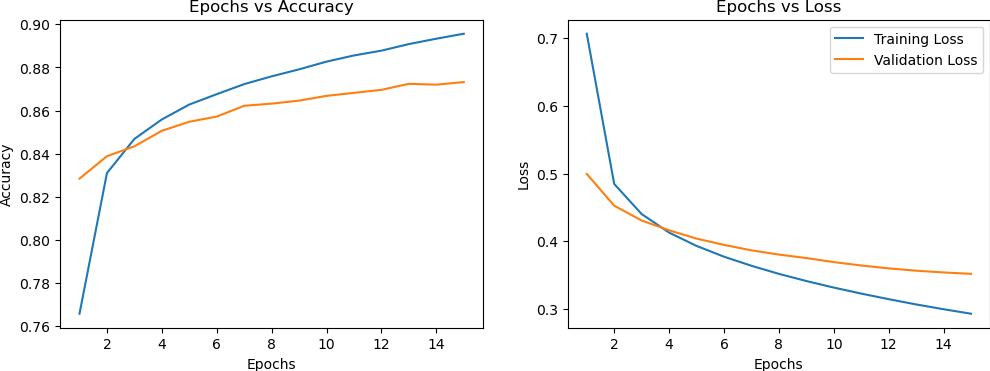
\includegraphics[width=\textwidth]{Fashion - Model 1.png}
        \end{subfigure}
        \begin{subfigure}[b]{0.48\textwidth}
            \centering
            \caption{$K$ Representative Images}
            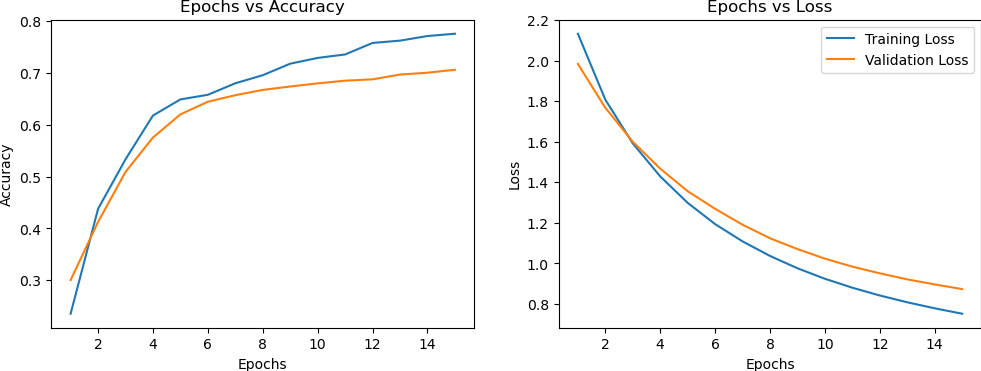
\includegraphics[width=\textwidth]{Fashion - Model 2.png}
        \end{subfigure}
        \begin{subfigure}[b]{0.48\textwidth}
            \centering
            \caption{Full Propagation}
            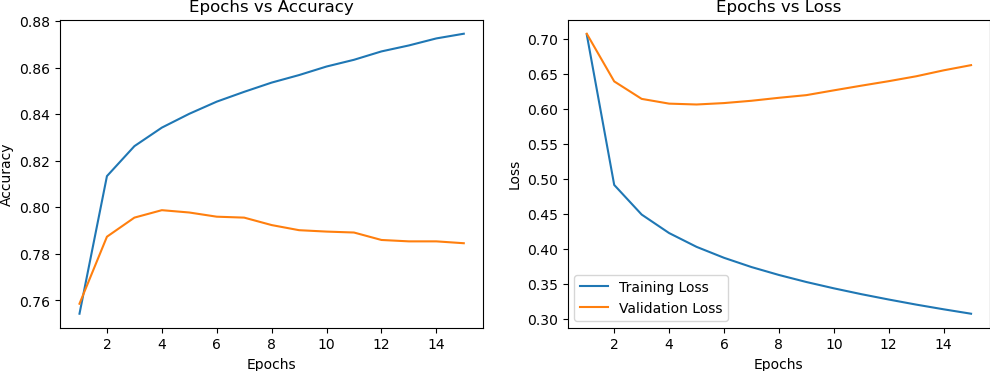
\includegraphics[width=\textwidth]{Fashion - Model 3.png}
        \end{subfigure}
        \begin{subfigure}[b]{0.48\textwidth}
            \centering
            \caption{Partial Propagation}
            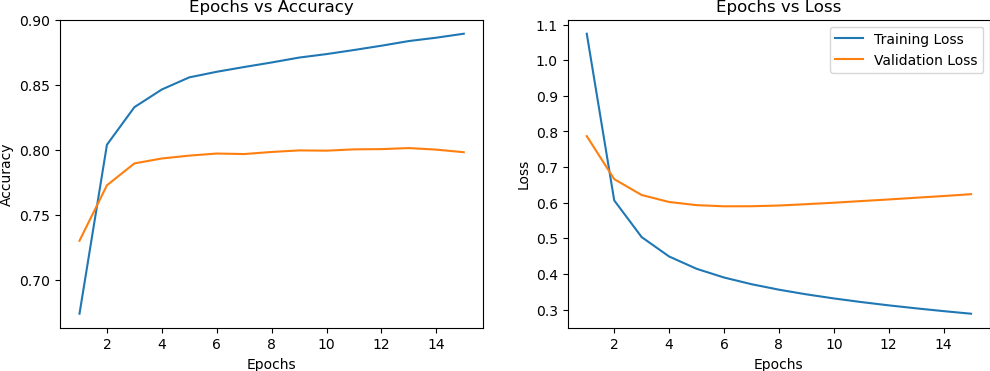
\includegraphics[width=\textwidth]{Fashion - Model 4.png}
        \end{subfigure}
    \end{figure}
    \begin{mdframed}
        Thus, we notice that for the Fashion MNIST Data, using the \emph{Original} Data (without any processing) is the best. Accuracy is the highest on the training and validation data, and the corresponding losses are the lowest. Furthermore, as clearly presented on the graphs, and mentioned in the table, metrics on the training and validation data are similar indicating that the model is not over-fitting.

        The processing of finding the \emph{$K$ Representative Images} reduces the accuracy but the similarity of the performance on the train and validation data indicates that the model is not over-fitting.

        The drastic difference in the performance on the train and validation data for the \emph{Full Propagated} and the \emph{Partially Propagated} data indicates that the model is over-fitting.
    \end{mdframed}
        
\subsection{Overhead}
  After clustering, optimal $k = 450$.
    \begin{table}[h]
        \begin{center}
            \begin{tabular}{|l|l|l|l|l|}
                \hline
                Model &Accuracy &Loss &Val-Accuracy &Val-Loss \\
                \hline
                Original &0.708 &0.844 &0.684 &0.905 \\
                $K$ Representative Images &0.456 &1.663 &0.277 &1.938 \\
                Full Propagation &0.727 &0.700 &0.381 &2.570 \\
                Partial Propagation &0.685 &0.834 &0.388 &1.935 \\
                \hline
            \end{tabular}
        \end{center}
    \end{table}
    \begin{figure}[!h]
        \centering
        \begin{subfigure}[b]{0.48\textwidth}
            \centering
            \caption{Original}
            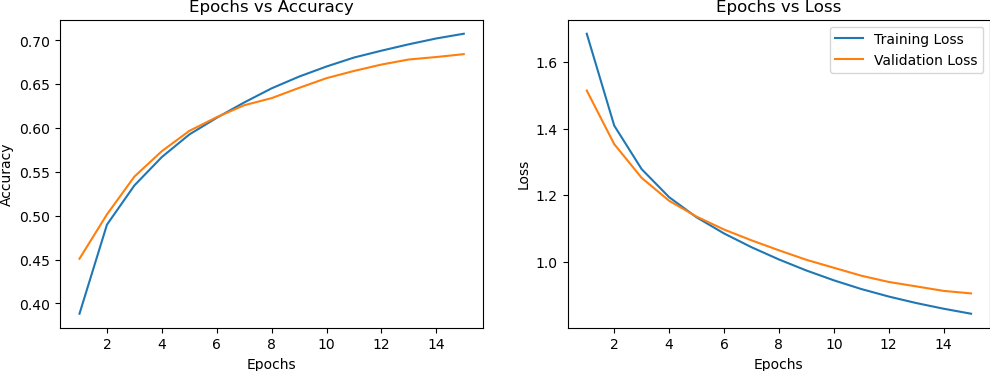
\includegraphics[width=\textwidth]{Overhead - Model 1.png}
        \end{subfigure}
        \begin{subfigure}[b]{0.48\textwidth}
            \centering
            \caption{$K$ Representative Images}
            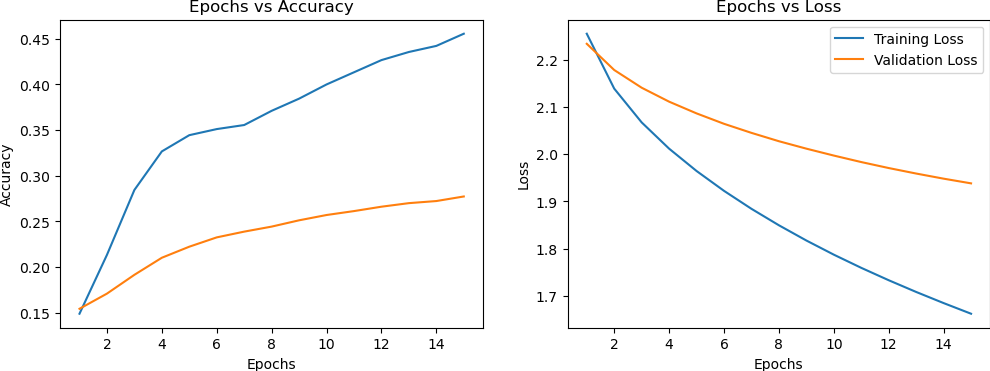
\includegraphics[width=\textwidth]{Overhead - Model 2.png}
        \end{subfigure}
        \begin{subfigure}[b]{0.48\textwidth}
            \centering
            \caption{Full Propagation}
            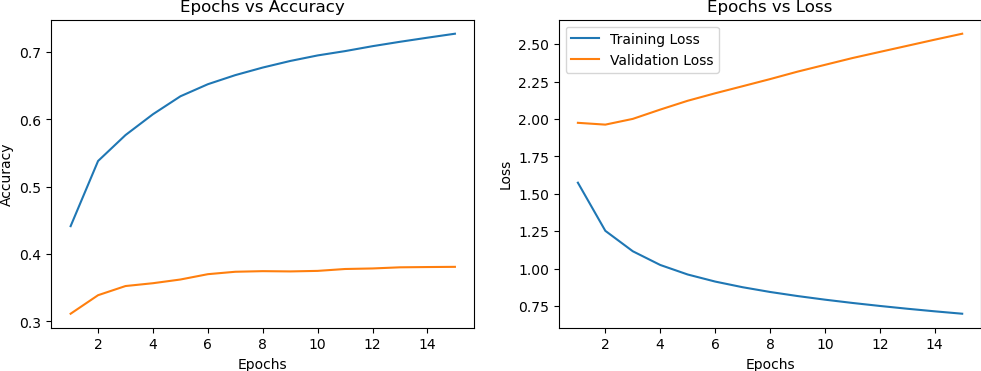
\includegraphics[width=\textwidth]{Overhead - Model 3.png}
        \end{subfigure}
        \begin{subfigure}[b]{0.48\textwidth}
            \centering
            \caption{Partial Propagation}
            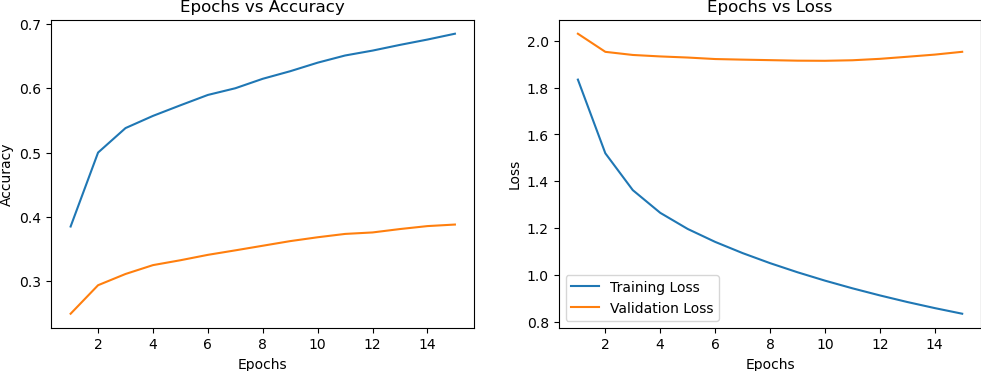
\includegraphics[width=\textwidth]{Overhead - Model 4.png}
        \end{subfigure}
    \end{figure}
    \begin{mdframed}
        Thus, we notice that for the Overhead Data, using the \emph{Original} Data (without any processing) is the best. Accuracy is the highest on the training and validation data, and the corresponding losses are the lowest. Furthermore, as clearly presented on the graphs, and mentioned in the table, metrics on the training and validation data are similar indicating that the model is not over-fitting.
        
        The drastic difference in the performance on the train and validation data for the \emph{$K$ Representative Images}, the \emph{Full Propagated} data and the \emph{Partially Propagated} data indicates that the model is over-fitting.
    \end{mdframed}
\end{document} % End of document body

